A highly used pattern in parallel computing is reduction. Reduction combines all elements in an array to a single element using an reduction operator. This can for example be used to calculate the sum or product of an array. In order for a reduction to work the reduction operator must be both binary and associative. Binary means that the operator is two-to-one, combining two element. Associative means that the order of which operations are performed does not effect the result, which can be mathematical expressed as \cref{def:reduce_associative}.

\begin{definition} 
\label{def:reduce_associative}
\textit{For an operator $\oplus$ to be associative the following statement must be true:}
\begin{center}
	$(a \oplus b) \oplus c = a \oplus (b \oplus c).$
\end{center}
\end{definition}

\noindent Addition and multiplication operators are associative while subtraction and division is not. The reduction can also be formally defined, which was done by Blelloch in \cite{BlellochTR90}, as seen in \cref{def:reduce}.

\begin{definition} 
	\label{def:reduce}
	\textit{The reduction operation takes a binary associative operator $\oplus$ with identity $\mathcal{I}$, and an ordered set}
	\begin{center}
		$[a_0, a_1,...,a_{n-1}]$ 
	\end{center}
	\textit{of $n$ elements, and returns the value}
	\begin{center}
		$a_0 \oplus a_1 \oplus ... \oplus a_{n-1}.$
	\end{center}
\end{definition}
\begin{example}
	\textit{For the binary associative operator $+$ and the ordered set}
	\begin{center}
		$[1,2,3,4,5,6,7,8]$ 
	\end{center}
	\textit{the return is}
	\begin{center}
		$36$
	\end{center}
	\end{example}

A visual representation of a serial reduction is seen on \cref{fig:reduce_serial}. 

\begin{figure}[ht]
	\centering
	\fbox{
		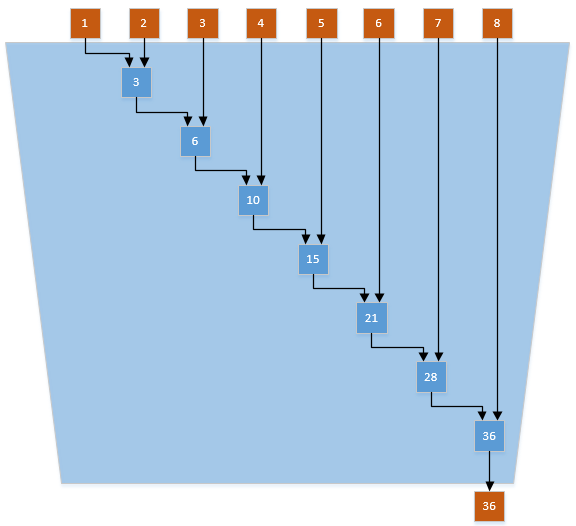
\includegraphics[width=0.5\textwidth]{figs/algorithm/reduce_serial.PNG}}
	\caption{Visual representation of the serial implementation of the reduction algorithm. The orange squares represent data elements, while the blue represent $\oplus$ operations}
	\label{fig:reduce_serial}
\end{figure}

Each operator operation in the serial implementation is data depend, which creates a chain of dependencies. The serial reduction is common for single core system and is commonly implemented using a loop. The step and work complexity for the serial reduction is $\mathcal{O}(n)$. Because of the data dependency in the serial reduction its operations cannot execute in parallel. A parallel reduction based on a binary tree is seen on \cref{fig:reduce_parallel}, here several of the operations can executed in parallel, thereby reducing the step complexity of the algorithm. 

\begin{figure}[ht]
	\centering
	\fbox{
		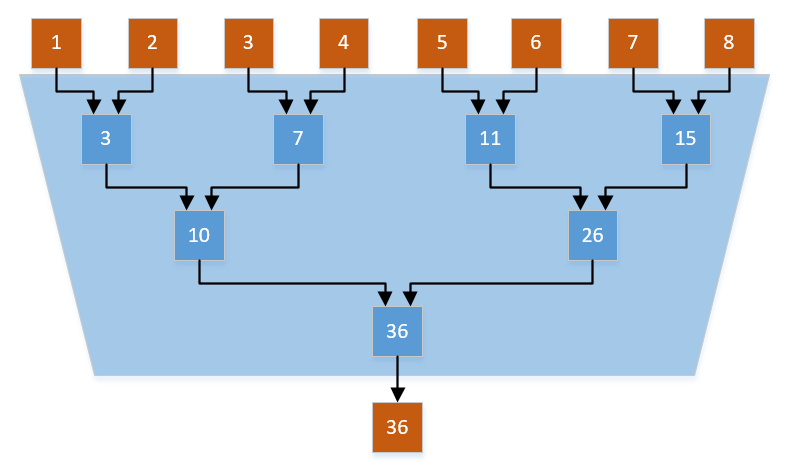
\includegraphics[width=0.6\textwidth]{figs/algorithm/reduce_parallel.png}}
	\caption{Visual representation of the parallel implementation of the reduction algorithm. The orange squares represent data elements, while the blue represent $\oplus$ operations}
	\label{fig:reduce_parallel}
\end{figure}

The binary tree parallel reduction has a work complexity of $\mathcal{O}(n)$ and a step complexity of $\mathcal{O}(log ~ n)$, thereby step efficient. 
The amount of data dependency is reduced, making it more suitable for parallel execution. A simple CUDA implementation of a reduction algorithm is seen in appendix \cref{ch:app_code_examples} in listing \ref{lst:reduce_kernel}. A fully working reduction can be found in \cite{exercises}. It should be noted that this example is not optimized, but is merely to show how a CUDA implementation looks. The shown implementation uses global memory and will only work on arrays smaller than the maximum threads per block. A way of making the reduce work on an arbitrary array size, is by combining multiple reductions as presented on \cref{fig:al_reduce_combine}:

\begin{figure}[ht]
	\centering
	\fbox{
		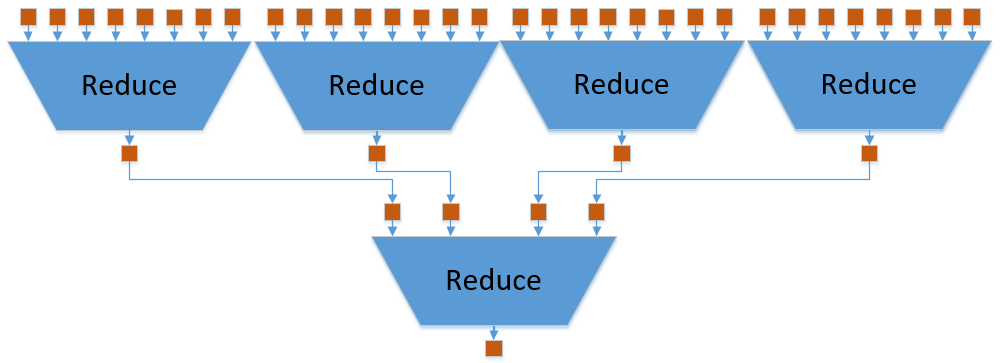
\includegraphics[width=0.9\textwidth]{figs/algorithm/reduce_combine.png}}
	\caption{Reduction using a reductions per thread block}
	\label{fig:al_reduce_combine}
\end{figure}

The combination of reductions enables reduction of both arbitrary array sizes and different array dimensions. Shared memory used by each  can also further optimize the reduction implementation.

The reduction algorithm is used in many application within parallel computing. An example of use is in Monte Carlo simulation, used in e.g. finance, computer graphics, image processing, where averages and variances of large arrays is needed.
